\documentclass[sn-nature,Numbered]{sn-jnl}

\usepackage{graphicx}
\usepackage{multirow}
\usepackage{amsmath,amssymb,amsfonts}
\usepackage{amsthm}
\usepackage{mathrsfs}
\usepackage[title]{appendix}
\usepackage{xcolor}
\usepackage{textcomp}
\usepackage{manyfoot}
\usepackage{booktabs}
\usepackage{algorithm}
\usepackage{algorithmicx}
\usepackage{algpseudocode}
\usepackage{listings}

\title[Article]{Transparency without pricing: a credit-level forensic account of collapse in the first tokenized carbon pool}

\author*[1]{\fnm{Wei} \sur{Cai}}\email{weicaics@uw.edu}

\author[1]{\fnm{Adeline} \sur{Wen}}\email{ywen8@uw.edu}

\begin{document}

\flushbottom
\maketitle

\affil*[1]{\orgdiv{Decentralized Computing Laboratory, School of Engineering and Technology}, \orgname{University of Washington Tacoma}, \orgaddress{\city{Tacoma}, \state{WA}, \country{USA}}}

\begin{abstract}
When assets of different quality are pooled and sold at a single price, theory predicts that low-quality units drive out high-quality ones, classically only when buyers cannot tell the difference. We document a collapse that occurred despite quality being fully and publicly observable, in a market whose design did not let price reflect it. We test this in the largest tokenized carbon-credit pool (22 million tonnes of CO$_2$), whose decline was widely blamed on low-quality forest credits. Analysing every deposit, withdrawal, and account on its public ledger, we find the opposite: 69\% renewable-energy credits with little additional climate benefit, and only 4\% of the blamed REDD+ forest credits. A few accounts extracted most of the high-value credits, while 9.3 million tonnes of low-value credits remain stranded to date. Identical credits placed in both a screened and an unscreened pool met sharply different fates, consistent with pool design, not credit type, shaping outcomes. Transparency alone therefore appears insufficient to prevent quality collapse: pooled markets may need to price quality, not merely disclose it, a caution for carbon policy and for the more than \$25-billion market now tokenizing other real-world assets on the same design.
\end{abstract}

\section*{Introduction}
Every year, companies and governments purchase carbon credits worth billions of dollars to offset their greenhouse gas emissions. A carbon credit represents one tonne of CO$_2$ prevented from entering the atmosphere, but the climate value of individual credits varies enormously. The central question for any carbon market is whether it can distinguish credits that represent genuine emission reductions from those that do not.

When market design fails to price quality differences, the result is adverse selection: a dynamic in which low-quality goods crowd out high-quality ones, first formalized by Akerlof in 1970 as the ``lemons problem''\textsuperscript{1,2,3}. The voluntary carbon market (VCM), whose annual transaction value peaked above \$2 billion in 2021--2022, faces exactly this risk. Fewer than 16\% of credits from investigated projects represent genuine reductions\textsuperscript{4}. At least 52\% of Indian wind power offsets went to projects that would have been built regardless of carbon revenue\textsuperscript{5}.

Blockchain-based tokenization promised to solve this problem through radical transparency. By recording every transaction on a public ledger, tokenized carbon pools would let any participant verify credit quality before trading. The first and largest such experiment was the Base Carbon Tonne (BCT) pool, operated by Toucan Protocol, which accepted verified credits from the Verra registry (the world's largest carbon-credit standard). Its key design feature: every accepted credit became an interchangeable token priced uniformly, regardless of underlying quality. The pool's value collapsed from a late-2021 peak above \$8 per tonne to \$0.71 by mid-2023, and to effectively zero by 2026.

Industry commentary and academic analyses attributed this collapse to low-quality forest conservation credits, specifically REDD+ (a program that pays landowners to avoid deforestation)\textsuperscript{2,6,7,8,9}. This narrative drew support from the broader literature documenting REDD+ crediting problems\textsuperscript{4,10,11}. But it was never tested against the pool's actual composition data, which are publicly recorded and straightforward to query. More broadly, no study has empirically tested the dominant policy assumption that transparency prevents quality collapse.

Here, we analyze every deposit (1,187), every recorded pool withdrawal (35,432; scored tokens), every credit token (161 individually scored, of 345 total), and every market participant (509 depositors, 28,897 redeemers) across BCT's operating history. The data contradict the prevailing narrative. BCT contained 69.1\% renewable energy credits (predominantly grid-connected hydropower, with wind and solar, registered across China, India, Turkey, and Brazil) with near-zero additionality (meaning the projects would have been built with or without carbon revenue), and just 4.2\% REDD+. A small number of accounts extracted most of the high-demand credits (1.55 million tonnes), while 9.3 million tonnes of low-quality credits remain stranded to date.

A comparison of identical credits across two pools with different quality screens sharpens the finding. The same credits were 100\% redeemed from BCT but only 28.5\% from a quality-gated pool, a contrast consistent with pool design, rather than credit type, shaping asset fate. Unlike prior work that quantifies overcrediting at the project level\textsuperscript{4,5,22,23}, we trace how overcredited assets are selectively extracted inside a pooled market even when quality is publicly observable.

We term this outcome \textit{design-enabled adverse selection}. It is distinct from Akerlof's classical lemons problem, which requires private information about quality. Here, quality information is available to all participants but is not reflected in prices. The pool treats every deposited credit as identical: a participant cannot buy a specific high-quality credit, only a generic pool unit priced at the pool average. We argue that uniform pricing of heterogeneous assets under voluntary participation is sufficient to produce market failure.

Because every transaction in this market is publicly recorded, its complete ledger supports the first credit-level forensic account of this dynamic, a reconstruction opaque off-chain markets cannot supply. We treat the market as a case study of a general prediction. The implication for pooled markets broadly, including the \$25-billion-plus tokenized real-world asset sector and the Article 6.4 crediting mechanism (the UN crediting mechanism under the Paris Agreement, operationalized at COP29 in 2024), is that transparency without price differentiation appears insufficient for market function.

\section*{Results}
\subsection*{BCT's real composition contradicts the REDD+ narrative}

We extracted all 1,187 deposit records from BCT's public transaction ledger, covering 168 unique Verra VCS (Verified Carbon Standard) projects and approximately 22 million tonnes of tokenized carbon credits (see Methods).

Renewable energy credits dominated the pool (Fig. 1). Grid-connected hydro, wind, and solar projects (predominantly from China and India, with Turkey and Brazil) registered between 2008 and 2013, constituted 69.1\% of total deposited tonnage. These are the categories from the CDM era (the Clean Development Mechanism, the Kyoto Protocol's now-wound-down UN crediting program, 2004--2020) that the ICVCM (Integrity Council for the Voluntary Carbon Market, the sector's main governance body) has declined to approve for its Core Carbon Principles (CCP) label. Multiple independent studies document their near-zero additionality: Cames et al.\textsuperscript{12} and Schneider\textsuperscript{13} in program-level assessments, Probst et al.\textsuperscript{4} in a meta-analysis finding no statistically significant emission reductions from wind power CDM projects, and Calel et al.\textsuperscript{5} estimating 52\% non-additionality among Indian wind offsets. The projects would have been built regardless of carbon revenue.



REDD+ credits, widely blamed for BCT's collapse, constituted just 4.2\% of the pool, more than sixteen times smaller than the renewable share. Even combining all nature-based categories (REDD+, ARR (afforestation, reforestation, and revegetation), and IFM (improved forest management)), the total reaches only 10\%, versus 69.1\% for renewables alone.


\subsection*{Base-rate selection: BCT over-selected renewables at 1.87$\times$ the registry rate}

BCT's renewable dominance could reflect the broader carbon credit supply rather than a selection effect. We obtained Verra VCS issuance data from MSCI (2024) and Ecosystem Marketplace (2023) indicating that renewables constitute approximately 37\% of total VCS issuance by volume (central estimate; robustness tested across the full sensitivity range of 26--48\%).

BCT's renewable share (69.1\% by tonnage) is 1.87$\times$ the VCS base rate (selection coefficient: the ratio of BCT's renewable share to the base rate; 1 = no over-selection). Because deposits cluster by account, we use account-clustered inference rather than a naive binomial test: an account-level permutation test (10,000 iterations) produces $p < 0.0001$, and 89.0\% of accounts hold majority-renewable portfolios. The over-selection is robust to conservative base-rate assumptions (remaining 1.44$\times$ at a 48\% null) and to account-level bootstrap and HHI-adjusted tests (Supplementary Methods).

Conversely, REDD+ is under-represented at 0.2$\times$ the VCS base rate (BCT 4.2\% vs. VCS $\sim$17\%), directly contradicting the narrative that REDD+ credits overwhelmed the pool.

\textbf{Bridge-level decomposition.} Toucan's bridge (the mechanism that moves an off-chain credit on-chain) passed essentially every Verra-bridged credit into BCT, 93.5\% of tokens and 99.6\% of tonnage (Supplementary Methods), so the 1.87$\times$ over-selection was a bridge-level phenomenon: the permissionless (open to anyone) bridge disproportionately attracted renewable credits from Verra, rather than depositors selecting them from a diverse universe. Pool-level selection space was essentially zero.


\subsection*{Price-quality feedback loop: composition predicts price collapse}

We next ask whether quality degradation drove the price collapse. We merged daily BCT prices in US-dollar terms (1,493 daily observations, October 2021 to July 2026; Methods) with daily cumulative quality metrics from the deposit stream ($n$ = 331 overlapping days).

\textbf{Correlation.} BCT's price falls as pool quality falls: price and the cumulative tonnage-weighted mean quality score are strongly correlated (Pearson $r$ = 0.77, $p < 10^{-66}$; equivalently $-$0.77 against PQD = 1 $-$ score/100; Methods; Fig.~2a). In a first-differenced OLS regression (analyzing day-to-day changes rather than levels, the credible specification for non-stationary series), each percentage-point increase in the renewable share of deposits predicts a \$0.018 decrease in BCT's price ($\beta$ = $-$1.8 on the 0--1 share, $p < 0.001$). Exploratory weekly Granger tests are asymmetric, dominant channel price to quality (Supplementary Methods).

\textbf{Redemption-side evidence.} Analysis of 35,432 Transfer events from the BCT pool contract reveals that selection operated on both sides. Non-renewable credits were preferentially redeemed: industrial gas 100\%, REDD+ 99.8\%, IFM 93.0\%, ARR 91.3\%, versus just 3.7\% of renewable credits. The tonnage-weighted mean composite quality score (0--100, higher = better) of redeemed credits (38.7) exceeded that of deposited credits (31.7) by 7 points, a 22\% premium. As a result, BCT's net renewable share increased from 71\% to 76\% over the pool's lifetime.

The exit followed a type-level Gresham sequence (bad drives out good): the most valuable credit types were extracted first, in an order matching off-chain market demand ($\rho$ = $-$0.74, $n$ = 7 types; Supplementary Methods). Before the May 2022 crash, redemptions targeted high-value credits (tonnage-weighted quality 42.0); afterwards quality dropped to 32.4, reflecting that the premium credits had been extracted while their off-chain value still exceeded BCT's redemption cost.

Depositors and redeemers are almost entirely distinct populations: only 1.4\% of 28,897 redeemer accounts also appear among the 509 depositor accounts. The top 10 redeemers account for 85.0\% of extracted tonnage. Their transactions occurred in rapid automated bursts (median gap 4.6 seconds), consistent with programmatic execution.

This dual-margin structure --- indiscriminate, architecture-driven entry (99.6\% tonnage pass-through) on one side; deliberate, type-specialist extraction on the other --- is not predicted by standard adverse-selection models, which assume a single population.


\subsection*{Account forensics: who extracted and what they took}

Account-level analysis of the 161 scored tokens' transfer histories reveals that the largest redeemers are type-specialist extractors who never participated in the deposit side.

\textbf{Table 1. Top 5 redeemers by tonnage.}

\begin{tabular}{lllll}
\toprule
Account & Tonnes redeemed & Dominant type & Mean quality & Also depositor? \\
\midrule
0x65a5... & 651,334 & Industrial gas & 30.9 & No \\
0x1b8e... & 335,556 & IFM & 40.0 & Yes \\
0xee4b... & 195,051 & REDD+ & 31.4 & No \\
0x4b3e... & 188,205 & ARR & 50.4 & No \\
0x8556... & 183,629 & ARR & 46.0 & No \\
\bottomrule
\end{tabular}
These five accounts removed 1.55 million tonnes: the vast majority of redeemed industrial gas, 37\% of REDD+, and 44\% of ARR. The largest by tonnage (0x65a5\ldots; 651,334 tonnes of industrial gas, 42\% of the 1.55 million) is not an arbitrageur but a smart contract, verified on-chain, that retired every credit in the same transaction as redemption (Data availability). That pattern is the signature of a retirement aggregator routing credits to final use. The other four are individual wallets whose redeem-then-hold behaviour is consistent with strategic arbitrage of the gap between BCT's uniform price and higher off-chain values, roughly \$7.4 million at midpoint price assumptions (\$10 million including the retirement contract; bounds \$0.3--\$22M; Methods). Fifteen of the twenty largest redeemers never deposited anything, and each targeted a single credit type.

Tracing each redeemed credit's immediate destination across the 20 largest extractors shows three pathways: cross-pool transfer to a quality-screened pool (NCT, Toucan's nature-restricted pool; 39.2\%), immediate retirement (34.6\%), and secondary-market sale (17.0\%). The cross-pool movement followed a systematic ordering (deposit, redeem, then re-deposit into the screened pool; Supplementary Methods).

Among the 399 accounts that both deposited and redeemed (the 1.4\% overlap population), a quality-swap analysis reveals no systematic quality arbitrage (Supplementary Methods). The dual-margin mechanism thus operates through largely distinct account populations connected by the pool's uniform pricing. A first-funder audit of the top 20 accounts per margin found entity-level links for a minority: one shared funding source, direct credit transfers among three accounts, and two dual-margin accounts, together 26\% of top-20 deposit and 9\% of top-20 redemption tonnage (Supplementary Table 5). The separation is therefore account-level, not entity-level.

\subsection*{Quality atlas and quality gating}

BCT's PQD of 0.679 places it at the bottom of the VCM quality spectrum, which spans a 10-fold range from 0.076 (DACCS, direct air carbon capture and storage) to 0.759 (grid-connected renewables) (Fig. 3). A within-pool permutation test ($z$ = $-$0.64, $p$ = 0.27) finds no evidence of within-pool selection bias; the eligible universe was uniformly low-quality. Letter grades B--AAA band the composite score; the BBB threshold separates credits with verified additionality from those without. Applied to the actual deposit stream, a BBB gate would have cut the deposit-weighted deficit from 0.689 to 0.506 while admitting only 7.2\% of deposited tonnage (Fig.~\ref{fig:gating}). The Toucan CHAR pool (biochar allowlist, PQD 0.221) is consistent with category restriction preventing quality collapse (Supplementary Fig. 2).


\subsection*{Temporal dynamics and robustness}

Deposit quality declines over BCT's operating life (Spearman $\rho$ = $-$0.24, $n$ = 1,187), but this is entirely a vintage-composition effect: late deposits drew from progressively older vintages (vintage, the credit's emission-reduction year), not from intrinsically worse credits within vintage (Supplementary Table 2). The May 2022 cryptocurrency crash provides exogenous deposit-side evidence of the causal channel: post-shock deposit quality fell 3.4 points (Cohen's $d$ = 0.49, a moderate effect) as volume collapsed by 98\% and the quality-decline slope tripled, consistent with the price-to-quality feedback above (Supplementary Methods).

\subsection*{Pool design and asset fate: a within-token cross-pool contrast}

A sharper contrast on the same data comes from 14 credit tokens (1.50 million tonnes) deposited into \textit{both} the unscreened pool (BCT) and the quality-screened pool (NCT), so the same physical credit appears under both designs with quality, vintage, registry, and project type held fixed. These 14 are the redeemed members of the 31 credits shared by the two pools, so the unscreened-side rate is near-universal (100\%) partly by this selection; the screened-side rate (28.5\%) is not symmetrically conditioned. The +73.9-percentage-point gap below is therefore best read as an upper bound on the contrast. Token by token (the unit of inference, $n$ = 14), the mean redemption gap is +73.9 percentage points (95\% CI [51, 93]; Fig.~\ref{fig:within_token}), unanimous in direction across every token and every credit type, with three exact tests (sign, permutation, Wilcoxon) returning $p$ = $2.4 \times 10^{-4}$. This is a two-pool contrast, not 14 independent treatments, and shares the two-pool confounds (exposure timing, liquidity, eligibility) that make the pool-level analysis descriptive only (Methods); its scope is also narrow, covering only nature-based credits. We therefore read it as \textit{strongly suggestive} of a pool-design effect rather than a proof, though robust: a hidden confounder would have to more than triple the odds that a credit is redeemed from one pool rather than the other to overturn the result (Supplementary Methods).

\textbf{Cross-pool comparison.} Recovering per-token credit identity on-chain for five pools across two operators (Toucan and C3, a second bridge protocol) and scoring each by our common framework, mean deposit quality rises monotonically with screening strictness, from the unscreened pools ($\sim$29--31) through nature-screened pools ($\sim$39--40) to the category-allowlist pool (77.9; Supplementary Table 4). This gradient is, however, definitional: a screen is defined on credit type and our composite is type-driven, so screened pools must score higher. A within-type check confirms the boundary: screened and unscreened pools hold nature-based credits of near-identical within-type quality (differences $\leq$0.32 points; Supplementary Methods), so screening acts on type, not within-type quality; the quantity is framework-derived (the C3 pools have no external validation). The unscreened pools also show a declining temporal slope absent in screened pools, but these raw slopes are not vintage-controlled (see the vintage drift above). We therefore read the cross-pool pattern as corroborative and descriptive only, not as evidence that design causes quality.


\subsection*{Market-revealed quality hierarchy}

Credit type alone, not the quality framework, captures the dominant axis of selective redemption: a framework-free type-only prediction rule out-predicts the quality-grade rule, and within the 116 renewable tokens neither vintage nor grade predicts redemption (Supplementary Table 3). The paper's core findings (composition, base-rate over-selection, redemption-side extraction, and the within-token cross-pool comparison) accordingly rest on transaction data and Verra credit-type classifications, not on the quality scoring framework (Supplementary Table 6).

In sum, 9.3 of 9.6 million deposited B-grade tonnes remain unredeemed (the scored analysis covers 15.2 million tonnes), among the largest carbon credit graveyards in existence.

\section*{Discussion}
Here, transparency without price differentiation did not prevent quality collapse; we argue it cannot in general. Every transaction was public and every credit's quality metadata freely available on the Verra registry and the blockchain. Yet the market collapsed exactly as economic theory predicts for markets with \textit{hidden} quality differences.

The underlying principle is Gresham's Law, which Akerlof (1970)\textsuperscript{1} generalized as the ``lemons problem'' for markets where quality is unobservable. BCT shows the same dynamic operates even when quality \textit{is} observable: the mechanism we term design-enabled adverse selection runs through market architecture rather than information asymmetry, identifying a distinct pathway to lemons-like outcomes. Our within-token contrast provides credit-level descriptive evidence consistent with the lemons dynamics that Manshadi et al.\textsuperscript{2} model theoretically.

Whenever heterogeneous assets are pooled at a single clearing price, with voluntary entry and exit, and the highest-quality units retain higher value outside the pool, those units are selectively withdrawn while low-quality units accumulate, \textit{independently of whether quality is observable}. Observability changes who profits from the spread, not whether the spread exists.

The misattribution of BCT's collapse to REDD+ credits\textsuperscript{7,8,9} illustrates how structural quality failures can hide in plain sight. CDM-era renewable energy credits constituted 69.1\% of BCT's tonnage. Their additionality was near zero because the projects were already economically competitive. Unlike REDD+ failures, which generate visible controversy over baselines (the hypothetical emission levels that would have occurred without the carbon credit project) and deforestation, the additionality failure of renewable energy credits is structurally invisible: the dams and wind farms exist, the electricity is real. Quality assurance frameworks that focus on high-profile failure modes may miss the categories that dominate pool composition.

Over nine million tonnes of nominally valid offsets remain stranded to date at a 97.6\% non-redemption rate (within the 161-token scored subset), an illustrative welfare gap with Monte Carlo median \$146M (90\% simulation interval \$68M--\$252M, parameter uncertainty only). Meanwhile, a small number of type-specialist accounts captured an estimated \$10 million at midpoint assumptions (an upper bound; Results) by selectively redeeming the credits that off-chain markets still valued, though the single largest such address is a retirement contract, not a profit-taking arbitrageur. The gap measures composition against a counterfactual pool; stranding concerns circulation; the frames are complementary. Paradoxically, BCT's failure functioned as an inadvertent quality filter, removing 9.3 million tonnes of low-quality credits from active circulation to date, an illiquidity event of a scale no registry-level intervention has achieved.

The underlying logic (Gresham's Law under uniform pricing) applies wherever heterogeneous assets are pooled\textsuperscript{3,14}. Six uniform-priced NFT vaults show the same entry-margin lemons selection, strongly in five and marginally in the sixth (deposited-item median percentiles 0.25--0.40 under strict sale matching, each $p < 10^{-10}$), with no exit-margin extraction in any. BCT, whose bridge passed heterogeneous credits wholesale, expressed selection at both margins (Supplementary Methods).

These findings apply most directly to voluntary pooling and registry-based bundling of credits, where quality-heterogeneous units clear at a common price\textsuperscript{14,15}. The Article 6.4 mechanism under the Paris Agreement is a registry-based crediting mechanism rather than a uniform-priced pool, so it inherits the design principle (price quality, or expect selection at any unpriced margin) rather than a direct prediction. Nor would gating alone have sufficed: even a minimal quality floor (composite score $\geq$29) would have excluded 58\% of BCT's tonnage. These results point to three design principles for future pooled crediting mechanisms: quality-differentiated pricing tiers rather than single-price pools; dual-margin gating of both deposits and withdrawals (exit-side extraction proved at least as damaging as entry-side quality loading); and dynamic quality floors that adjust as composition shifts. Our findings are consistent with, and lend urgency to, the ICVCM's Core Carbon Principles framework\textsuperscript{16}. The emerging quality-differentiation ecosystem (Singapore's integration of independent ratings into eligibility assessments\textsuperscript{17}, blockchain credibility indices\textsuperscript{18}) must incorporate dual-margin design to be effective; we release the three principles as an open-source reference implementation\textsuperscript{19} (on-chain registry and gate, off-chain monitor script; $\approx$19k gas; Supplementary Methods).

The same public data also support a deployable early-warning. A cumulative Lemons Index (0--1, higher = worse average pool quality), computed in real time from deposits already observed, crossed its 0.50 danger threshold at the pool's launch, at 0.71 near the \$5.66 launch level, roughly seven months before the price fell below half that level. A framework-free variant, the cumulative renewable share, exceeded its own threshold permanently from the pool's first week (Supplementary Methods). Because this is a standing \textit{level} signal, it does not depend on price history: the diagnostic information was in the composition from inception (exploratory temporal-ordering tests are reported in Supplementary Methods). Paired with the quality gate above (0.689 to 0.506 at a BBB floor, 7.2\% of tonnage admitted; Fig.~\ref{fig:gating}), this converts the post-mortem into an actionable protocol: audit composition at inception, gate deposits and redemptions on quality, and re-audit as the pool evolves.

Several limitations warrant note. Our quality scores are author-derived, but the core findings rely on transaction data and Verra credit-type classifications, not on the scoring framework. The framework itself is calibrated against CCP labels ($d$ = 1.8; Fig.~\ref{fig:ccp}), commercial ratings ($\rho$ = +0.901, $n$ = 27; non-blind, scored with agency ratings in view; Supplementary Fig. 1), and a large-language-model panel (Fleiss' $\kappa$ = 0.6, moderate agreement; Supplementary Methods). Both cross-pool comparisons are descriptive, not causal identifications. The within-token contrast (+73.9 pp gap, $\Gamma$ = 3.05 bound) and the pool-level difference-in-differences rest on only two pools; their statistics quantify per-pair variability, not the pool-level confounds (exposure timing, liquidity, eligibility) that remain collinear with the screening label (Methods). We read the contrast as strongly suggestive of a pool-design effect, noting that the dominant renewables are structurally excluded from this nature-based comparison. The bridge decomposition (99.6\% pass-through by tonnage) establishes that entry-side selection was primarily architectural rather than strategic.

This result carries a falsifiable policy implication: any pooled crediting system providing quality transparency without quality-differentiated pricing will experience the same collapse. The transparency reforms by the ICVCM and the Article 6.4 Supervisory Body are necessary but not sufficient: if Article 6.4 pools heterogeneous credits at a single price, the same Gresham dynamic should emerge, and mechanisms with quality-differentiated tiers should not. This prediction is testable as Article 6.4 becomes operational.

The tokenized real-world asset sector now exceeds \$25 billion and is replicating pool-based architecture across commodities, bonds, and receivables. BCT is the first pool to complete a full quality-collapse cycle with auditable transaction data. Its lesson is straightforward: quality-differentiated mechanism design is not an optional refinement for pooled carbon markets but a structural prerequisite for market integrity.

\section*{Methods}
Full methods are provided in Supplementary Methods; this section summarizes the essentials.

\textbf{Data.} All 1,187 deposits to the BCT pool (October 2021 to late 2022; 168 Verra VCS projects, 345 TCO2 tokens, approximately 22 million tonnes) and all 708 NCT deposits were collected from Polygon via RPC, with transaction, depositor, token, project, vintage, and tonnage recorded. Projects were cross-referenced against the Verra registry for methodology category, country, and CCP status, and classified into eleven methodology categories (tonnage-weighted statistics). Redemptions are ERC-20 Transfer events with the pool as sender (35,432 events across the 161 originally scored tokens). Daily BCT prices (1,493 observations, October 2021 to July 2026) come from the DeFi Llama API via the committed \texttt{fetch\_bct\_prices.py}.

\textbf{Quality scoring.} A composite score (0--100) weights six dimensions: removal type (0.250), additionality (0.200), MRV (0.200), permanence (0.175), vintage (0.100), and registry/methodology (0.075), derived from the Oxford Offsetting Principles\textsuperscript{20} and the ICVCM CCP Assessment Framework\textsuperscript{16}; grades AAA--B are threshold bands, and seven disqualifiers cap grades. The Pool Quality Deficit is PQD = $1 - \bar{C}/100$ (tonnage-weighted). The cumulative deposit-weighted PQD, computed in real time, is the Lemons Index used for early warning. Weight perturbation (10,000 Dirichlet samples) leaves 93.7\% of grades unchanged.

\textbf{Selection tests.} The base-rate selection coefficient $S = f_{\text{BCT}} / f_{\text{VCS}}$ (central base rate 37\%, sensitivity range 26--48\%) is tested with account-clustered inference. The within-token contrast treats the 14 tokens deposited into both BCT and NCT as their own controls, tested with three exact procedures and a percentile bootstrap; the estimand is the pool-design effect on dual-eligible credits, and a Rosenbaum-style $\Gamma$ quantifies robustness to unobserved confounding. A deposit-level difference-in-differences and a five-pool, two-operator comparison are reported as descriptive corroboration only.

\textbf{Price, cross-domain, and welfare.} A first-differenced OLS with Newey--West errors tests price-quality co-movement ($n$ = 330 days); weekly Granger tests ($n$ = 55) are exploratory. The NFTX cross-asset pipeline assigns each minted or redeemed item the percentile of its nearest sale within a drift-controlled window of collection sales, testing entry-margin selection per vault (Wilcoxon) and across vaults (sign test), with router accounts excluded. The welfare gap is a 10,000-iteration Monte Carlo propagating literature additionality ranges\textsuperscript{4,12,22,23}, the social cost of carbon (\$50--\$200/tCO$_2$), and a base-rate counterfactual composition.

\textbf{Inference.} All $p$-values were corrected using the Benjamini--Hochberg FDR procedure at $\alpha$ = 0.05 across ten primary tests: (1) base-rate selection coefficient (account-clustered; naive binomial as reference only), (2) full-sample and (3) pre-shock temporal correlations, (4) the within-token sign test, (5) the pool-level difference (descriptive), (6--7) bidirectional Granger, (8) within-pool permutation, (9) depositor concentration, and (10) the redemption differential (token-level Mann--Whitney; $n$ = 161). Cluster-robust bootstrap (by depositor account, 10,000 iterations) was used for deposit-level statistics.

\subsection*{Data availability}

All data, scoring rubrics, analysis scripts, and smart contract source code are available at \url{https://github.com/Adeline117/carbon-neutrality} (version tag \texttt{v1.0-erl-submission} pins the state cited here) under an MIT licence. Machine-readable rubrics are in JSON format. The 318-credit methodology batch dataset with per-dimension scores is included. All 345/345 BCT tokens are scored (161 original + 184 imputed). On-chain deposit data for both BCT (1,187 transactions) and NCT (708 transactions) are provided with transaction hashes enabling independent verification. The externally-owned-account versus smart-contract status of the top redeemers was checked with \texttt{eth\_getCode} against a public Polygon node; results are recorded in \texttt{redeemer\_contract\_check.json}. The entity-level independence audit (first-funder resolution for the top 20 accounts per margin) is reproducible via \texttt{entity\_funding\_analysis.py}, with per-wallet results in \texttt{entity\_funding\_analysis.json}. LLM panel outputs for all models across 29 credits are included. Analysis scripts are pure Python with NumPy/SciPy as sole dependencies; a single verification script (\texttt{tools/verify\_headline\_numbers.py}) re-asserts every headline number against the cached analysis outputs.


\subsection*{Code availability}

All analysis code is available at https://github.com/Adeline117/carbon-neutrality under an MIT licence.

\subsection*{Author contributions}

A.W. designed the study, collected and analyzed all data, developed the quality scoring framework, performed all statistical analyses, and wrote the manuscript. W.C. supervised the research and provided critical revisions.

\subsection*{Competing interests}

The authors declare no competing interests.

\subsection*{Acknowledgements}

This research received no specific grant from any funding agency. The authors thank the Decentralized Computing Laboratory at the University of Washington Tacoma for computational resources and discussion.

\begin{thebibliography}{21}
\bibitem{1} Akerlof, G. A. The market for ``lemons'': quality uncertainty and the market mechanism. \textit{Q. J. Econ.} \textbf{84}, 488--500 (1970).
\bibitem{2} Manshadi, V. H. et al. Offsetting carbon with lemons: adverse selection and certification in the voluntary carbon market. SSRN Working Paper (2025).
\bibitem{3} Battocletti, V. et al. The voluntary carbon market: market failures and policy implications. \textit{Colo. Law Rev.} \textbf{95}, 519--572 (2024).
\bibitem{4} Probst, B. et al. Systematic assessment of the achieved emission reductions of carbon crediting projects. \textit{Nat. Commun.} \textbf{15}, 9562 (2024).
\bibitem{5} Calel, R. et al. Do carbon offsets offset carbon? \textit{Am. Econ. J. Appl. Econ.} \textbf{17}, 1--40 (2025).
\bibitem{6} Berg, F. et al. The market for voluntary carbon offsets. SSRN Working Paper (2025).
\bibitem{7} Bassi, E. et al. Blockchain-based voluntary carbon market: strategic insights into network structure. \textit{Front. Blockchain} \textbf{8}, 1603695 (2025).
\bibitem{8} Ballesteros-Rodriguez, A., De-Lucio, J. \& Sicilia, J. Tokenized carbon credits in voluntary carbon markets: the case of KlimaDAO. \textit{Front. Blockchain} \textbf{7}, 1474540 (2024).
\bibitem{9} Jirasek, M. KlimaDAO: a crypto answer to carbon markets. \textit{J. Organ. Des.} \textbf{12}, 271--283 (2023).
\bibitem{10} Trencher, G. et al. Demand for low-quality offsets by major companies undermines climate integrity of the voluntary carbon market. \textit{Nat. Commun.} \textbf{15}, 6863 (2024).
\bibitem{11} West, T. A. P. et al. Action needed to make carbon offsets from forest conservation work for climate change mitigation. \textit{Science} \textbf{381}, 873--877 (2023).
\bibitem{12} Cames, M. et al. How additional is the Clean Development Mechanism? Oko-Institut Report (2016).
\bibitem{13} Schneider, L. Assessing the additionality of CDM projects: practical experiences and lessons learned. \textit{Clim. Policy} \textbf{9}, 242--254 (2009).
\bibitem{14} World Bank. State and Trends of Carbon Pricing 2025. World Bank Group (2025).
\bibitem{15} Garcia, A. \& Sanford, L. On the potential for strategic behavior in jurisdictional REDD+. \textit{Proc. Natl Acad. Sci. USA} \textbf{123}, e2531612123 (2026).
\bibitem{16} Integrity Council for the Voluntary Carbon Market. Core Carbon Principles, Assessment Framework, and Assessment Procedure. ICVCM (2023).
\bibitem{17} Singapore National Environment Agency. Carbon rating panel: appointment of BeZero, Calyx Global, and Sylvera. NEA Regulatory Notice (2025).
\bibitem{18} Gao, H. O., Liu, X. et al. A blockchain-based carbon registry platform for credible climate action in transportation. \textit{npj Clim. Action} \textbf{5}, 23 (2026).
\bibitem{19} Reference implementation: composable quality-rating registry and gated pools (Solidity/Foundry). \url{https://github.com/Adeline117/carbon-neutrality} (contracts/), MIT licence.
\bibitem{20} Allen, M. et al. The Oxford Principles for Net Zero Aligned Carbon Offsetting. University of Oxford (2020).
\bibitem{21} MSCI. State of integrity in the global carbon-credit market. MSCI ESG Research (2024).
\bibitem{22} Badgley, G., Freeman, J., Hamman, J. J., Haya, B., Trugman, A. T., Anderegg, W. R. L. \& Cullenward, D. Systematic over-crediting in California's forest carbon offsets program. \textit{Glob. Change Biol.} \textbf{28}, 1433--1445 (2022).
\bibitem{23} Haya, B. K. et al. Comprehensive review of carbon quantification by improved forest management offset protocols. \textit{Front. For. Glob. Change} \textbf{6}, 958879 (2023).
\end{thebibliography}


\clearpage

\begin{figure}[ht]
\centering
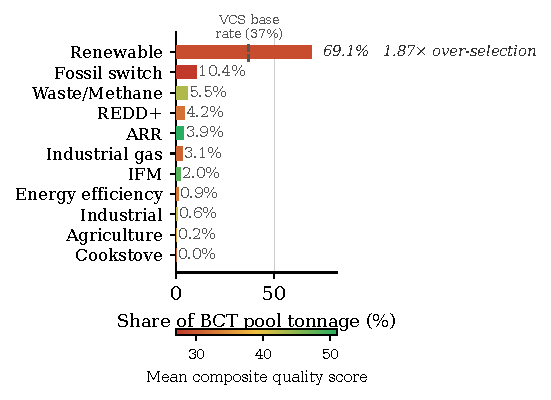
\includegraphics[width=\textwidth]{../../../figures/fig1_composition.pdf}
\caption{BCT pool composition by methodology category, weighted by deposited tonnage. Renewable energy credits constitute 69.1\% of total deposited tonnage; REDD+ constitutes just 4.2\%.}
\label{fig:composition}
\end{figure}

\begin{figure}[ht]
\centering
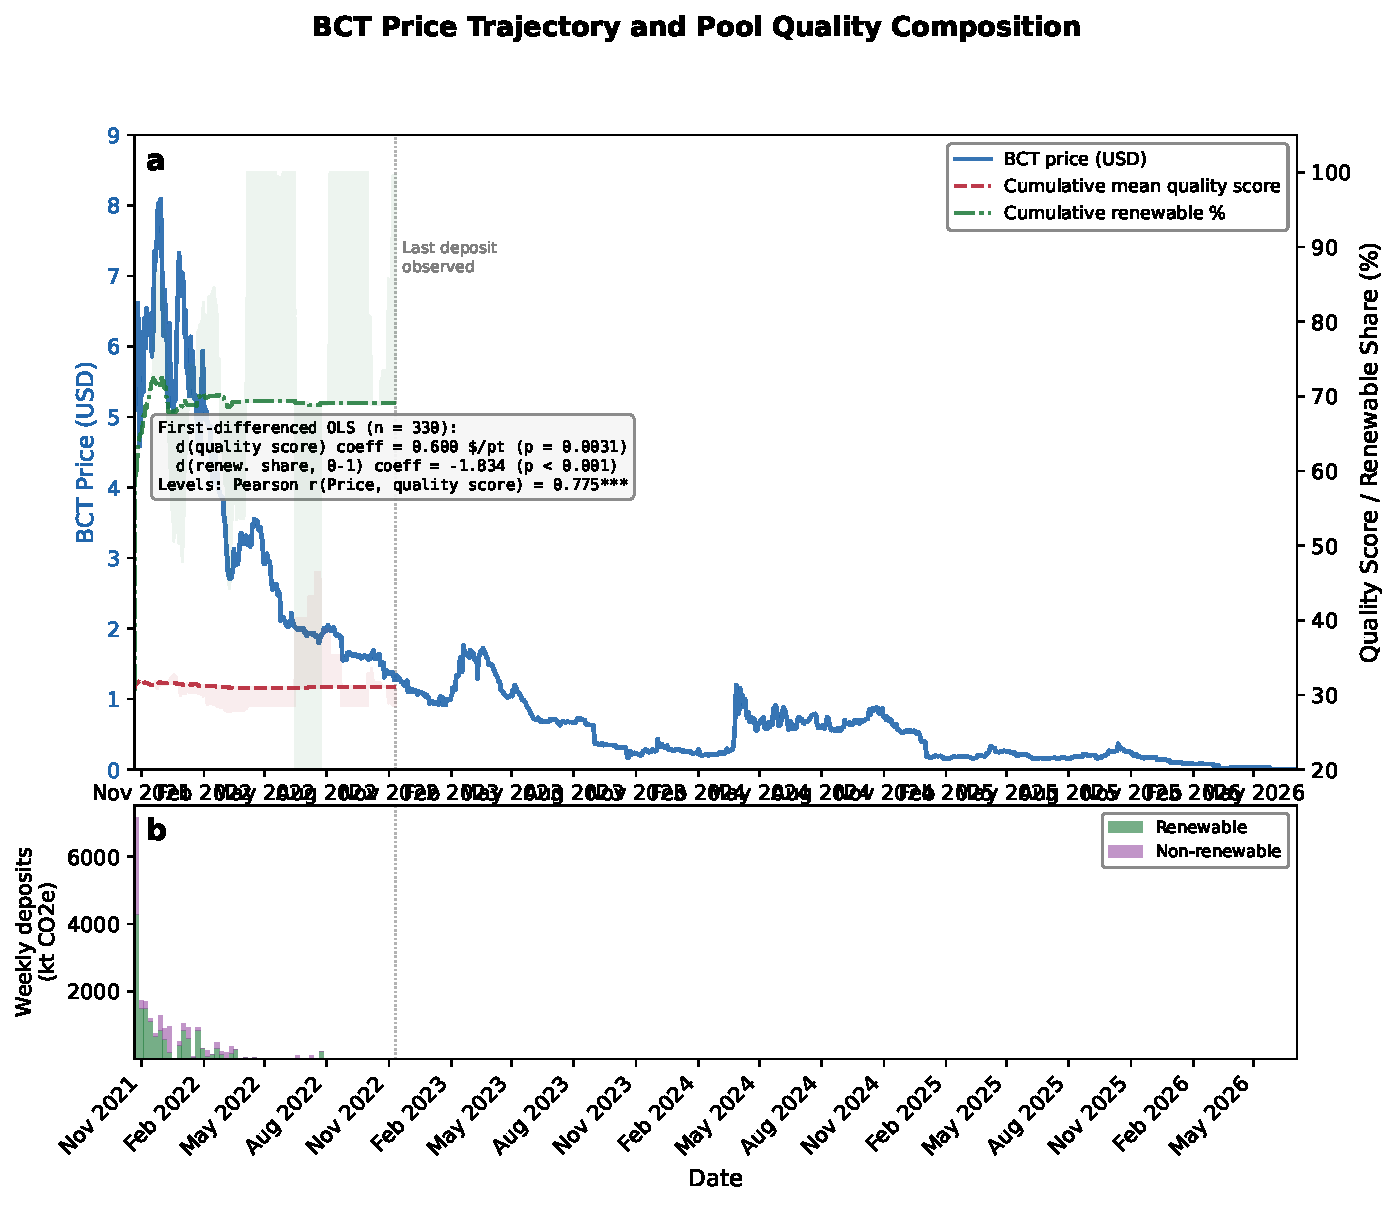
\includegraphics[width=\textwidth]{../../../figures/fig2_price_quality.pdf}
\caption{BCT price trajectory and pool quality composition. (\textbf{a}) Daily BCT price against cumulative Pool Quality Deficit and cumulative renewable share; inset reports the first-differenced OLS ($n$ = 330) and the levels correlation (Pearson $r$ = 0.774). (\textbf{b}) Weekly deposit volume split into renewable and non-renewable tonnage.}
\label{fig:price_quality}
\end{figure}

\begin{figure}[ht]
\centering
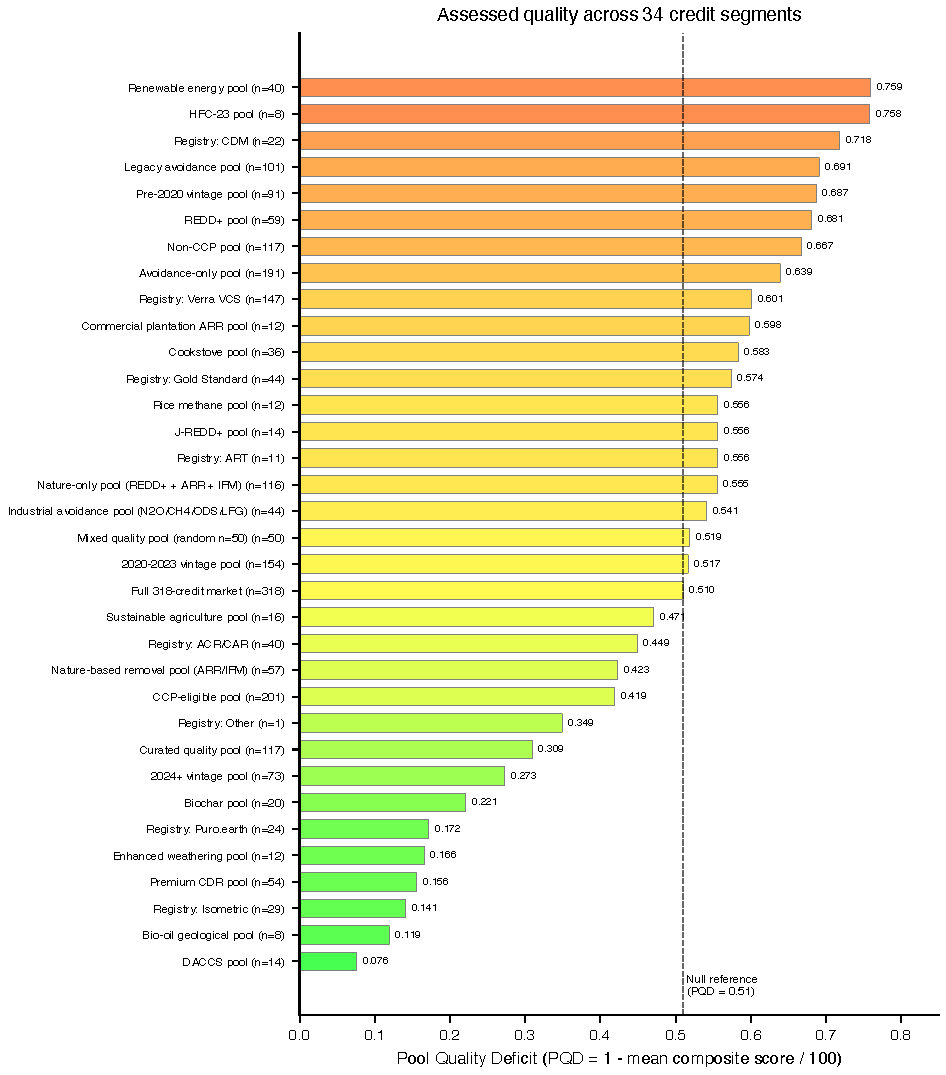
\includegraphics[width=\textwidth]{../../../figures/fig3_quality_atlas.pdf}
\caption{Quality atlas: 34-segment PQD spectrum with null model baseline. PQD ranges from 0.076 (DACCS) to 0.759 (grid-connected renewables).}
\label{fig:quality_atlas}
\end{figure}

\begin{figure}[ht]
\centering
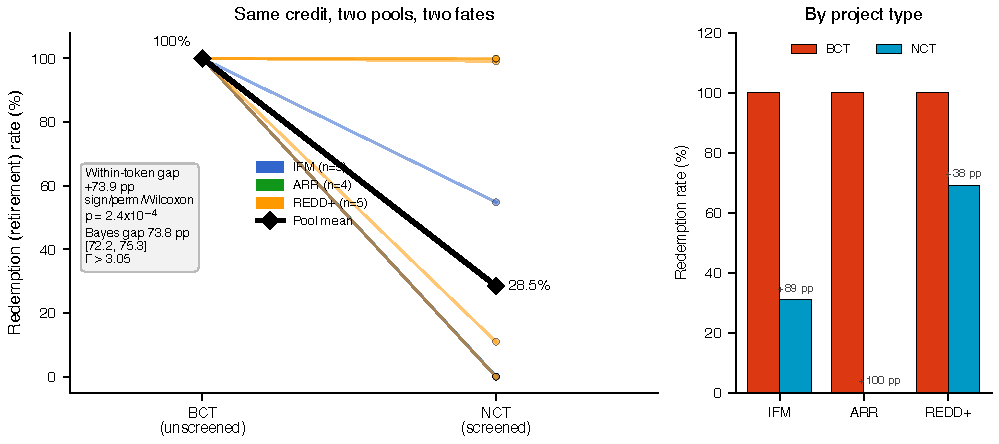
\includegraphics[width=\textwidth]{../../../figures/natcomms_fig_within_token.pdf}
\caption{Within-token cross-pool contrast: redemption of identical credits under two pool designs (descriptive; a two-pool comparison, not a causal identification). (\textbf{a}) Per-token slope plot of redemption (retirement) rate for the 14 carbon credit tokens deposited into \textit{both} the unscreened BCT pool and the quality-screened NCT pool, coloured by project type; the bold black line traces the pool means (100.0\% redeemed from the unscreened pool versus 28.5\% from the screened pool). Across the 14 pairs (the unit of inference) the mean within-token redemption gap is +73.9 percentage points (token-level bootstrap 95\% CI [51, 93]); the direction is unanimous, so exact sign, permutation, and Wilcoxon tests all return $p$ = $2.4 \times 10^{-4}$ whether or not the one near-tied credit is included. (\textbf{b}) Redemption rate by project type (bars: tonnage-weighted rates; annotated gaps: per-token mean differences): the gap is positive within every type (IFM +89, ARR +100, REDD+ +38 pp per-token). The result is robust to unobserved confounding up to a Rosenbaum bound of $\Gamma$ = 3.05. Depositor-level temporal, base-rate, and difference-in-differences robustness analyses are reported in Supplementary Methods.}
\label{fig:within_token}
\end{figure}

\begin{figure}[ht]
\centering
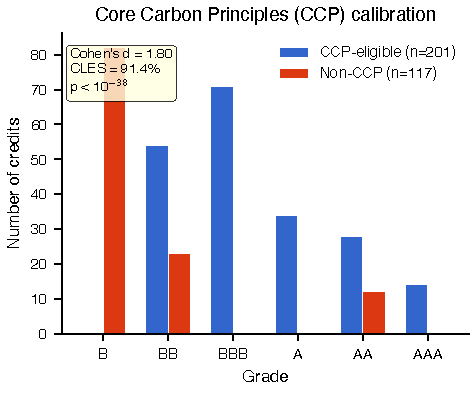
\includegraphics[width=\textwidth]{../../../figures/fig5_ccp_calibration.pdf}
\caption{CCP calibration: quality score distributions for CCP-eligible versus non-CCP credits. Cohen's $d$ = 1.8 (95\% CI [1.5, 2.16]).}
\label{fig:ccp}
\end{figure}

\begin{figure}[ht]
\centering
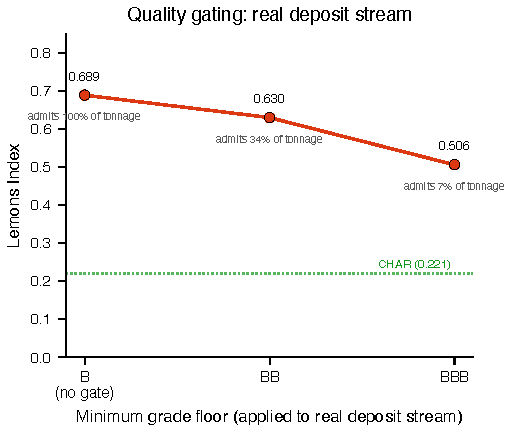
\includegraphics[width=\textwidth]{../../../figures/fig6_quality_gating.pdf}
\caption{Quality gating applied to the real BCT deposit stream: gated Lemons Index and admitted tonnage share under grade floors (B = no gate, BB, BBB). A BBB floor cuts the deposit-weighted Lemons Index (PQD) from 0.689 to 0.506 but admits only 7.2\% of deposited tonnage; the CHAR category-allowlist pool (0.221) is shown for reference.}
\label{fig:gating}
\end{figure}



\end{document}
